\documentclass[11pt,a4paper]{ivoa}
\usepackage[top=1in, bottom=0.75in, left=0.85in, right=0.85in]{geometry}
\usepackage{hyperref}
\usepackage{listings}
\DefineNamedColor{named}{keyword}{rgb}{.5,0,.3}
\DefineNamedColor{named}{comment}{rgb}{0.25,0.5, 0.37}
\DefineNamedColor{named}{string}{rgb}{0.16,0.0, 1.0}

\lstdefinelanguage{vodsl}{
    language = Java,
    alsodigit = {-},
    keywords = {model,author,include,package,abstract,primitive,dtype,otype,as,ordered,composition,enum,references,semantic,subset,iskey,ofRank}   
}
\lstdefinelanguage{xtext} {
    language = Java %FIXME define xtext
}

\lstset{
    language=vodsl,
    basicstyle=\small\ttfamily,
    keywordstyle=\color{keyword},
    commentstyle=\color{comment},
    stringstyle=\color{string},
    showstringspaces=false,
    tabsize=3
}
\input tthdefs
\input gitmeta
\vcsurl{https://github.com/pahjbo/vodsl}

\title{VODSL: a Domain Specific Language for VO-DML}

% see ivoatexDoc for what group names to use here; use \ivoagroup[IG] for
% interest groups.
\ivoagroup{Data Models}

\author[https://wiki.ivoa.net/twiki/bin/view/IVOA/PaulHarrison]{Paul Harrison}

\editor{Paul Harrison}

% \previousversion[????URL????]{????Concise Document Label????}
\previousversion{This is the first public release}
       

\begin{document}
\begin{abstract}
VOSDL is a compact domain specfic language with the sole purpose of creating data models that are expressed in VO-DML. The aim is to make
it easier for a team of authors to develop data models. This is achieved by creating a simple source code that
is amenable to being managed easily in version control systems.
\end{abstract}


\section*{Acknowledgments}

The \emph{Virtual Observatory (VO)} is a
general term for a collection of federated resources that can be used
to conduct astronomical research, education, and outreach.
The \href{https://www.ivoa.net}{International
Virtual Observatory Alliance (IVOA)} is a global
collaboration of separately funded projects to develop standards and
infrastructure that enable VO applications.


\section{Introduction}

VO-DML is the IVOA standard language for creating data models and the standard document  \cite{2018ivoa.spec.0910L} details the reasons behind its
creation and the advantages of using such a language over other more general languages such as UML. The standard representation of VO-DML is XML and as such
it is difficult to edit model instances directly, especially as the XML is a direct representation of the VO-DML meta model. The most common practice envisaged by the
standard is that data models are generally created by visual UML tools and then the UML converted to VO-DML via the XMI interchange format. This approach does work,
but it has several disadvantages.

\begin{enumerate}
\item UML tools tend to have poor interoperability despite the standard XMI interchange format \begin{itemize}
  \item There needs to be a specialized XMI $\Rightarrow$ VO-DML conversion written for each UML tool (and sometimes for each version of a particular tool).
  \item It is difficult to ``import'' an existing VO-DML definition into a particular UML tool.
\end{itemize}
\item Because of this poor interoperability between UML tools it is difficult for authors to collaborate on the creation of a data model \begin{itemize}
  \item even if they are using the same tool and use XMI in a version control system, there is
  \item if they are using different UML tools, comprehending what might be small incremental changes in the source becomes impossible.
\end{itemize}
\item Commercial UML tools tend to be expensive, and the free ones less feature rich.
\end{enumerate}

These difficulties were the inspiration for creating VODSL as a new route to producing VO-DML with the following characteristics;
\begin{itemize}
\item Text based for easy management by version control systems.
\item Concise, so that it is easy for direct comprehension by humans.
\end{itemize}

The VODSL language and its associated tools are version controlled in \href{https://github.com/pahjbo/vodsl}{GitHub} as well
as some \href{https://github.com/ivoa/vodsl-models}{examples} of 
models expressed in VODSL.

\subsection{Relationship to VO-DML}
\label{sec:relation}

\begin{figure}
\centering
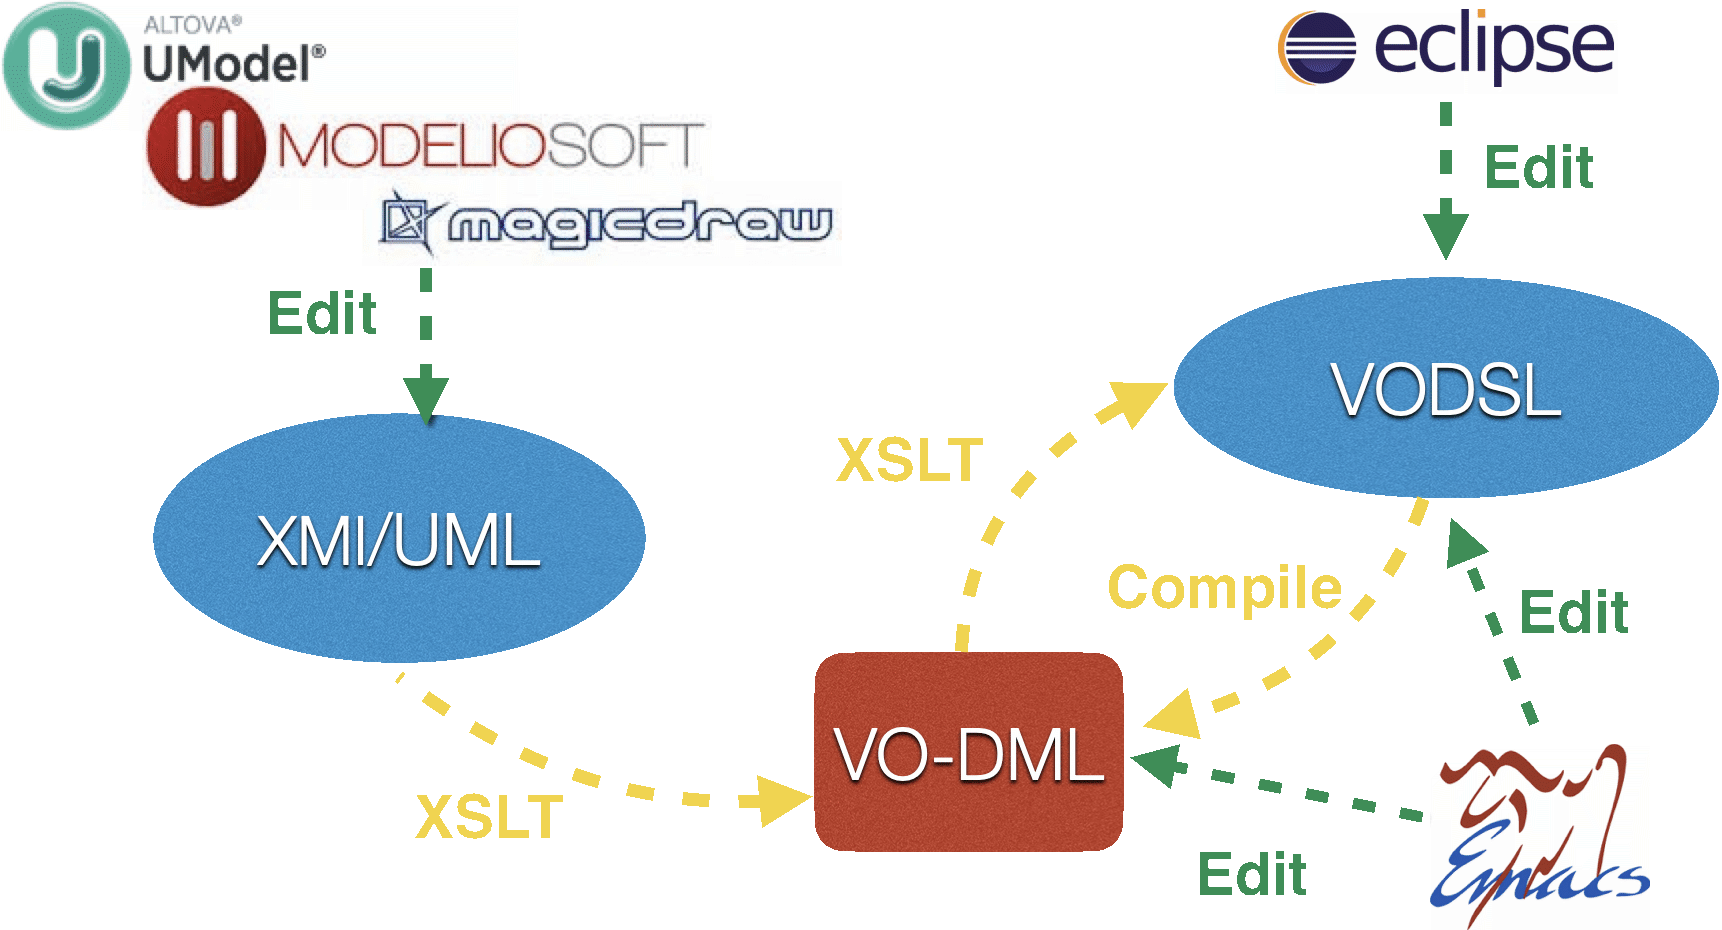
\includegraphics[width=\textwidth]{ecosystem.png}
\caption{How VODSL fits in the VO-DML ecosystem}
\label{fig:ecosystem}
\end{figure}

Fig.~\ref{fig:ecosystem} shows the role that VODSL plays in the VO-DML creation ecosystem - The yellow arrows indicate transformations that can
be made programatically between the different formats, and the green arrows indicate ways in which the source can be edited and the tools that can be
used to create or edit that particular representation. It shows that VODSL has a similar role to XMI/UML in the creation of VO-DML, although with one
significant advantage in that there is an exact transformation VO-DML$\Rightarrow$VODSL.

\begin{table}
\begin{tabular}{p{0.4\textwidth}p{0.1\textwidth}p{0.4\textwidth}}
VODSL&& UML \\
\hline
Easier to perform global refactoring & vs & Easier to visualise the whole model \\
Instant validation\footnote{when using the Eclipse plug-in} & vs & Full validation only after XSLT transformation of XMI \\
Easier to merge contributions from two authors textually & vs & Rely on UML tool to have model merging facility \\
\end{tabular}
\caption{VODSL route vs UML route}
\label{table:comparison}
\end{table}

\section{VODSL language}


The VODSL language use the same underlying meta-model as VO-DML (see the grammar in \label{sec:grammar}), but uses a mapping to a syntax that makes it easier
for humans to write by hand. It uses a general C/Java-like syntax with the following characteristics;

\begin{itemize}
  \item pairs of curly braces representing grouping
  \item attribute declarations ending with semi-colons \lstinline{;}
  \item line comments introduced by \lstinline{// comment}
  \item block comments \lstinline{/* comment */}
  \item keywords \begin{lstlisting}
  model,author,include,package,abstract,primitive,dtype,
  otype,as,ordered,composition,enum,references,semantic,
  subset,iskey,ofRank
  \end{lstlisting}
  \item attibute names precede their types
  \item \lstinline{"documentation strings"} are enforced for all types
  \item multiplicities are introduced by \lstinline{@}
\end{itemize}

The syntax of various parts of the language are described in the following sections. For a fuller description of the 
semantics of the language, the VO-DML standard itself should be consulted.


\subsection{Model Declaration}
The model declaration includes the name of the model its version followed by a description and then a number of authors.
\begin{lstlisting}[language=vodsl]
 model example (0.1) "description here" 
   author "Paul Harrison"
   author "An Other"
   
   include "IVOA-v1.0.vodsl"

\end{lstlisting}

It will almost always be the case that there should be an include statement that includes the standard IVOA VO-DML base model which defines a 
number of fundamental primitive types. There can be additonal includes to re-use parts of other models.

\subsection{Packages}
Packages may be used to partition the namespace in a model. Is is not required that all definitions live in a package as there is an assumed ``unnamed'' 
which exists at the top-level of the model. Packages may be nested.
\begin{lstlisting}[language=vodsl]
package p "package" {
	package n "nested package" {
   
	}
}
\end{lstlisting}

Note that the above fragment is not actually legal without the inner package containing a type definition.

\subsection{Types}

Types are defined by starting with the particular type keyword. Where appropriate this might be preceded by \lstinline{abstract} and
if the type is a sub-type of another type then after the type name the supertype is indicated with \lstinline{->}.

\begin{lstlisting}
abstract otype ad1 -> base "an abstract subtype "{	
}
\end{lstlisting}

\subsubsection{Primitives}
\begin{lstlisting}[language=vodsl]
primitive angle "another primitive"
\end{lstlisting}
note the lack of a semi-colon at the end of this declaration.

\subsubsection{Enumerations}
\begin{lstlisting}[language=vodsl]
enum options "an enum" {
	val1 "first option",
	val2 "second option"
}   

\end{lstlisting}

\subsubsection{DataTypes}

DataTypes are defined with the ``dtype'' keyword. This definition also introduces the syntax for attribute definitions, which are defined between the curly
braces of the main DataType definition.
\begin{lstlisting}[language=vodsl]
dtype myQuant -> ivoa:RealQuantity "a flagged quantity" {
			flag : ivoa:boolean "the flag" ;
}

\end{lstlisting}



\subsubsection{ObjectTypes}
ObjectTypes are defined with the ``otype'' keyword.
\begin{lstlisting}[language=vodsl]
otype o1 {
	     /* the following attribute is a 'natural key' for the otype */
	       name : ivoa:string iskey "the identifier";
			   bv : ivoa:anyURI  "Description";
		    /* note use of ^ to be able to 
		            re-use reserved word.*/	
		    ^author: ivoa:string "author"; 
}

\end{lstlisting}

This definition also introduces the \lstinline{iskey} attribute modifier to hint to any code generation systems that this attribute should be regarded as a
``natural key'' for the ObjectType and used rather than generating a surrogate key.

\subsubsection{Multiplicities}
\begin{lstlisting}[language=vodsl]
otype multiplicities "the @ sign introduces a multiplicity"
{
	m1 : ivoa:integer @? "0 or 1";
	m2 : ivoa:integer @* "0 or many";
	m3 : ivoa:integer @+ "1 or many";
	m4 : ivoa:integer @[2] "twice (as an array?)";
}

\end{lstlisting}

\subsubsection{References and Compositions}

This example shows the syntax for references and compositions and the difference in their semantics.
\begin{lstlisting}[language=vodsl]


 /*  this referred to otype is not affected by the lifecycle
   of other instances in the model */
 otype ReferedTo { 
 	test1: ivoa:integer "";
 }

/* instances of this contained class will only live
   as long as the containing instance.  */
otype Contained  {
 	test2: ivoa:string "";
 }
 
otype RCTest { 
	ref references ReferedTo "";
	contained : Contained @+ as composition "";
}

\end{lstlisting}


\subsubsection{Subsetting}
Subsetting is an advanced VO-DML feature, where an attribute of a subtype can be declared to be a particular sub-type of the supertype's attribute type.
\begin{lstlisting}[language=vodsl]

otype subs -> base {
	/* note that the requirement to refer to the q attribute of base */
   subset base.q as myQuant; //the type of base.q is a supertype of myQuant
}
\end{lstlisting}



\subsection{Scoping}

Type names need to be brought into scope by including the model where they are defined, and thereafter they can be referred to by prefixing the type name with
the model name followed by a colon. Types defined in the same model as where they are referred to do not need this model prefix.

If the type is futher namepspaced by packages, then to refer to a type in a package the enclosing package names should be separated by periods. The use of a period to separate name parts
is also necessary when referring to an attribute of a type - e.g.\ when subsetting.\footnote{The eclipse plugin has a small bug in that it will sometimes make the first separation of a name
reference with a colon even when the referred to type is in fact in the same model}

\section{VODSL tools}
The tools associated with the VODSL language are being developed in a GitHub repository \url{https://github.com/pahjbo/vodsl} and use \href{https://eclipse.org/Xtext}{XText}
to implement the language itself as well as the Eclipse integration. 

\subsection{Eclipse plugin}

\begin{figure}
\centering
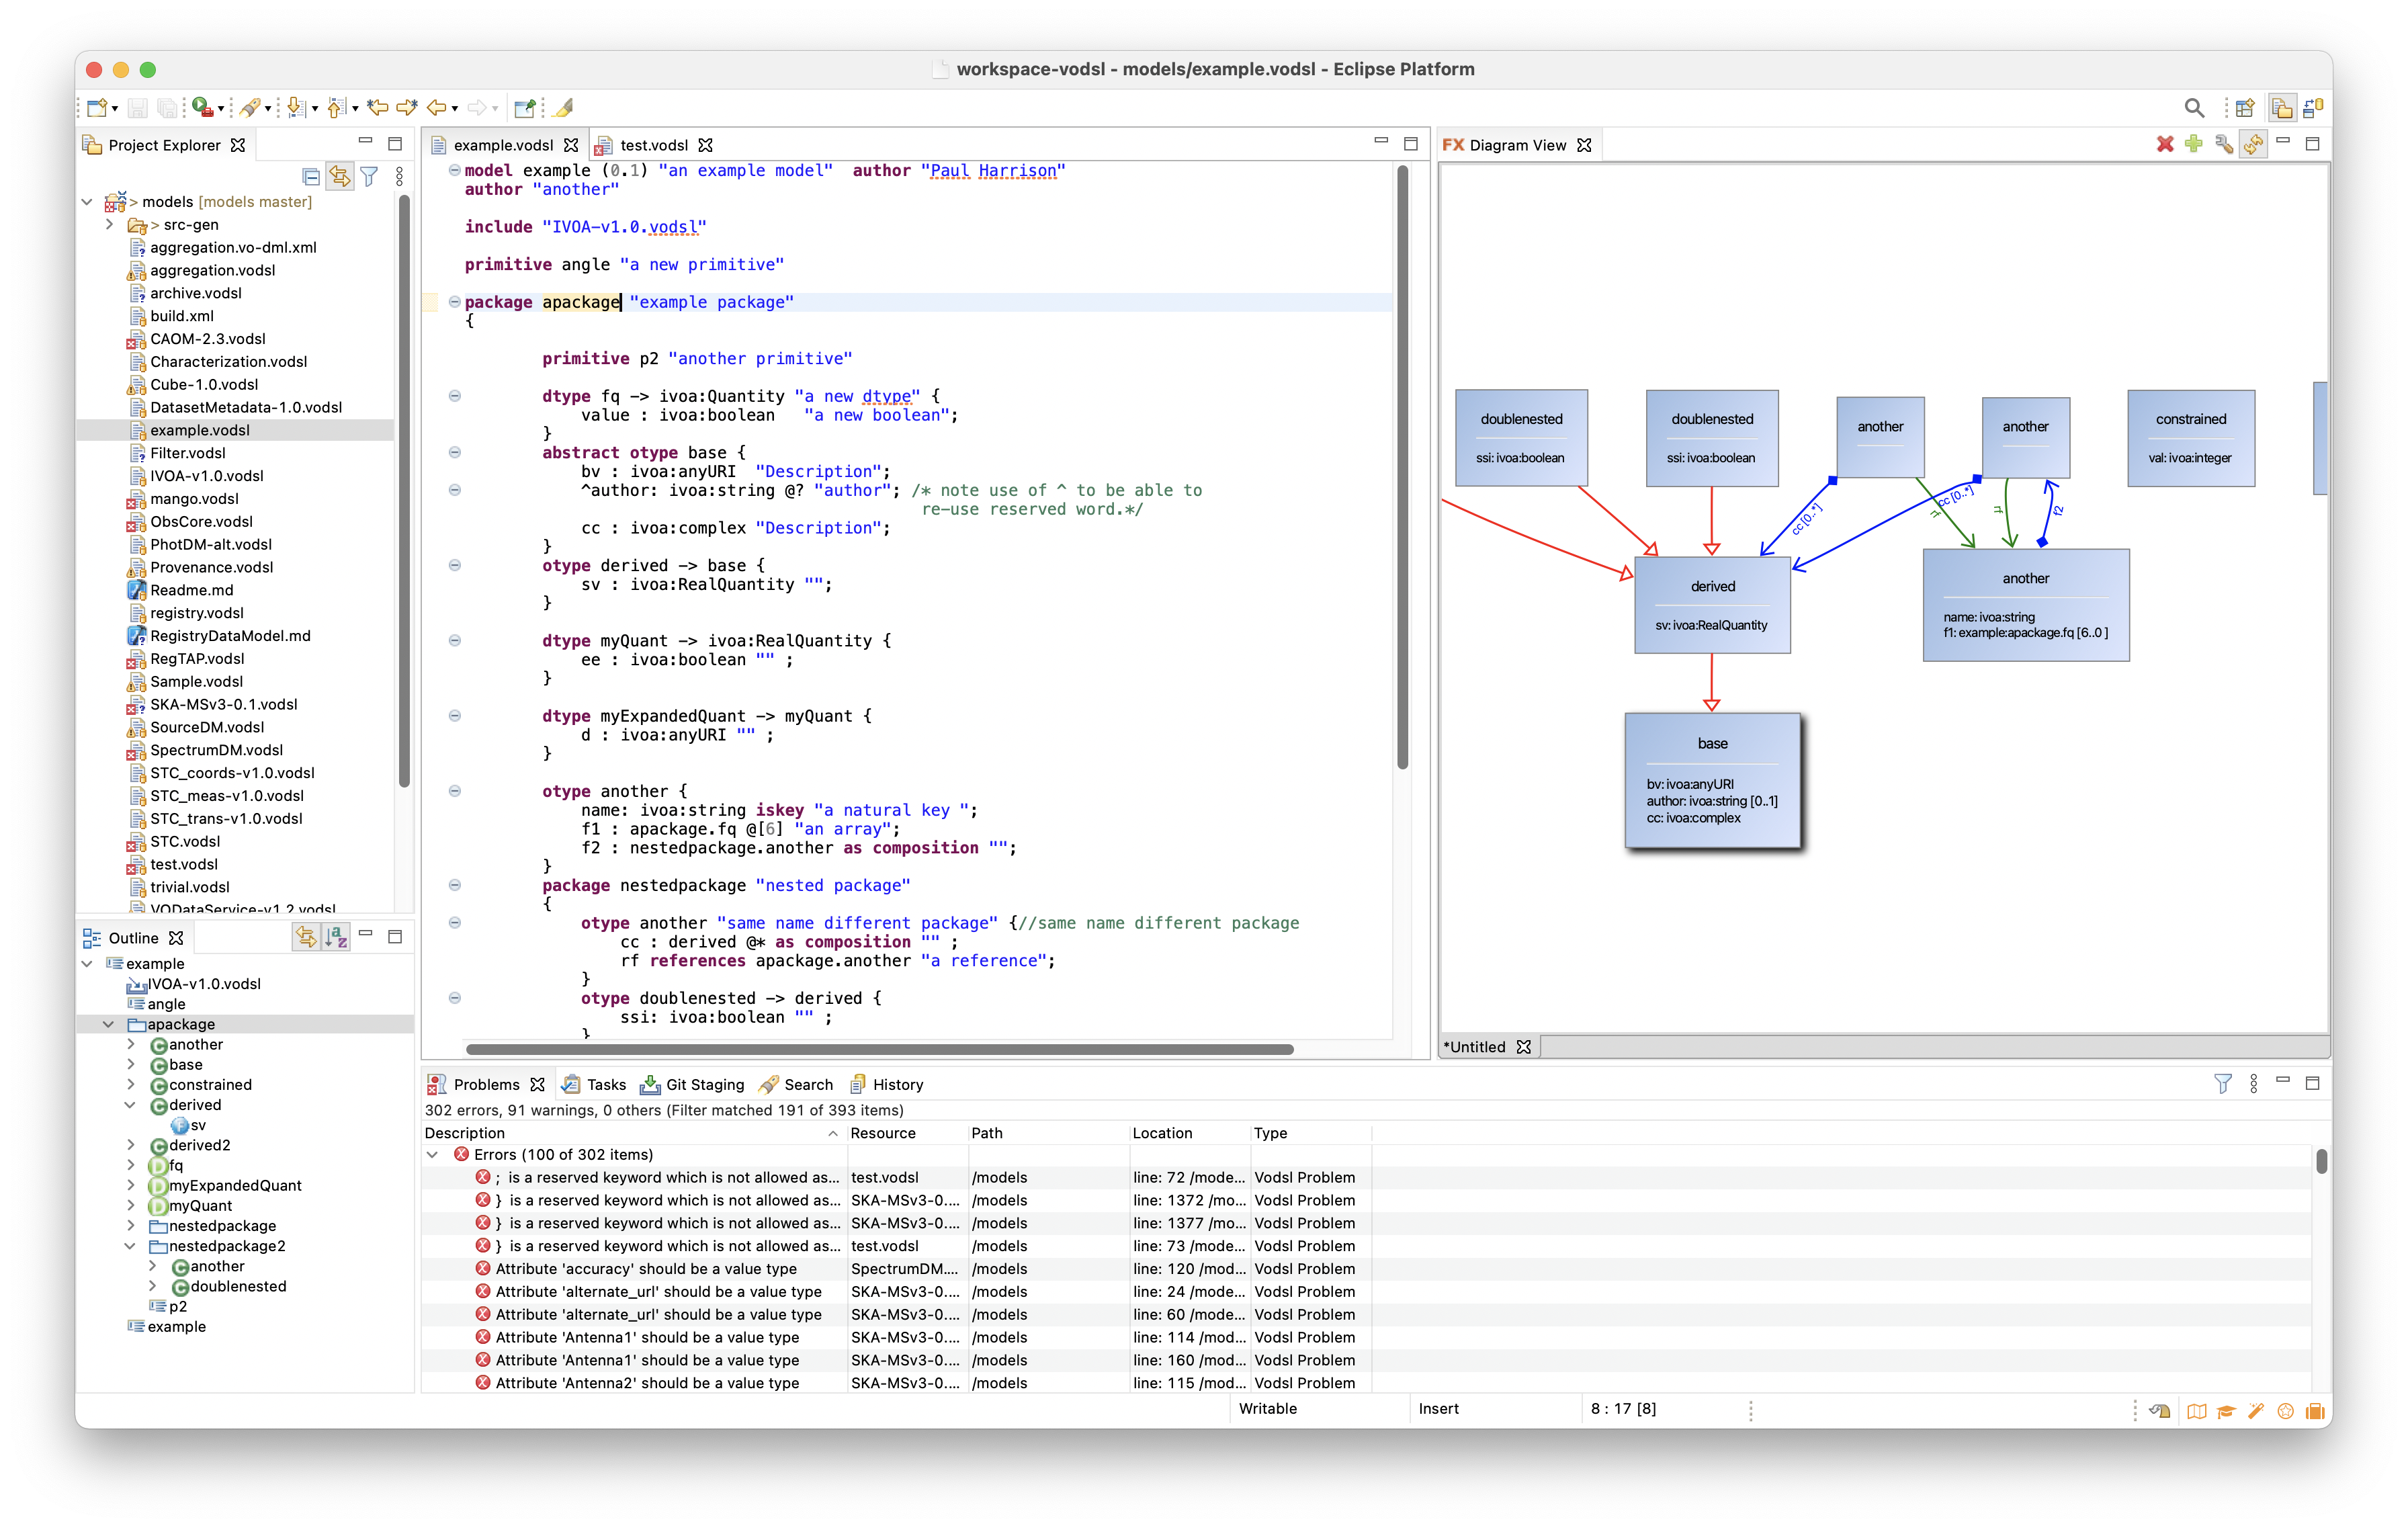
\includegraphics[width=\textwidth]{eclipsevodsl.png}
\caption{Eclipse running the VODSL plugin}
\label{fig:eclipsevodsl}
\end{figure}


Although it is possible to edit VODSL with any plain text editor as discussed in \ref{sec:relation}, an Eclipse plug-in has been 
created (Fig.~\ref{fig:eclipsevodsl} shows a screenshot of Eclipse running the plugin) that allows VOSDL source to be edited whilst
 taking advantage of the all the features of the Eclipse that make understanding an navigating the code
easier. As well as the expected IDE conveniences of syntax colouring, context sensitive suggestions and ease of navigation,
 the most important feature of the plug-in are;

\begin{itemize}
  \item Compilation of VODSL to VO-DML.
  \item Real-time validation and syntax checking.
  \item Navigation via a graphical representation of the model.
\end{itemize}

\subsubsection{VODSL compilation}

The plugin will compile any VODSL it finds (files with `.vodsl` extension) 
to the output directory specified in the compiler section of the VODSL preferences. 
The compilation will occur whenever the enclosing project is built, and if ``build automatically''
is set then this will be every time that the VODSL file is saved.

\subsubsection{The Graphical View}
 
The graphical view of the model is implemented in \href{http://jankoehnlein.github.io/FXDiagram/}{FXDiagram} and uses some of the same
conventions as the standard graphical representation produced by the VO-DML tools, i.e.\ 
\begin{itemize}
  \item subclass relations are represented by red connectors
  \item reference relations are represented by green connectors
  \item composition relations are represented by blue connectors
\end{itemize}

The graphical view is opened by right clicking on one of the 
declarations in the text view of the model and selecting ``Show in FXDiagram $\Rightarrow$ VODSL model''

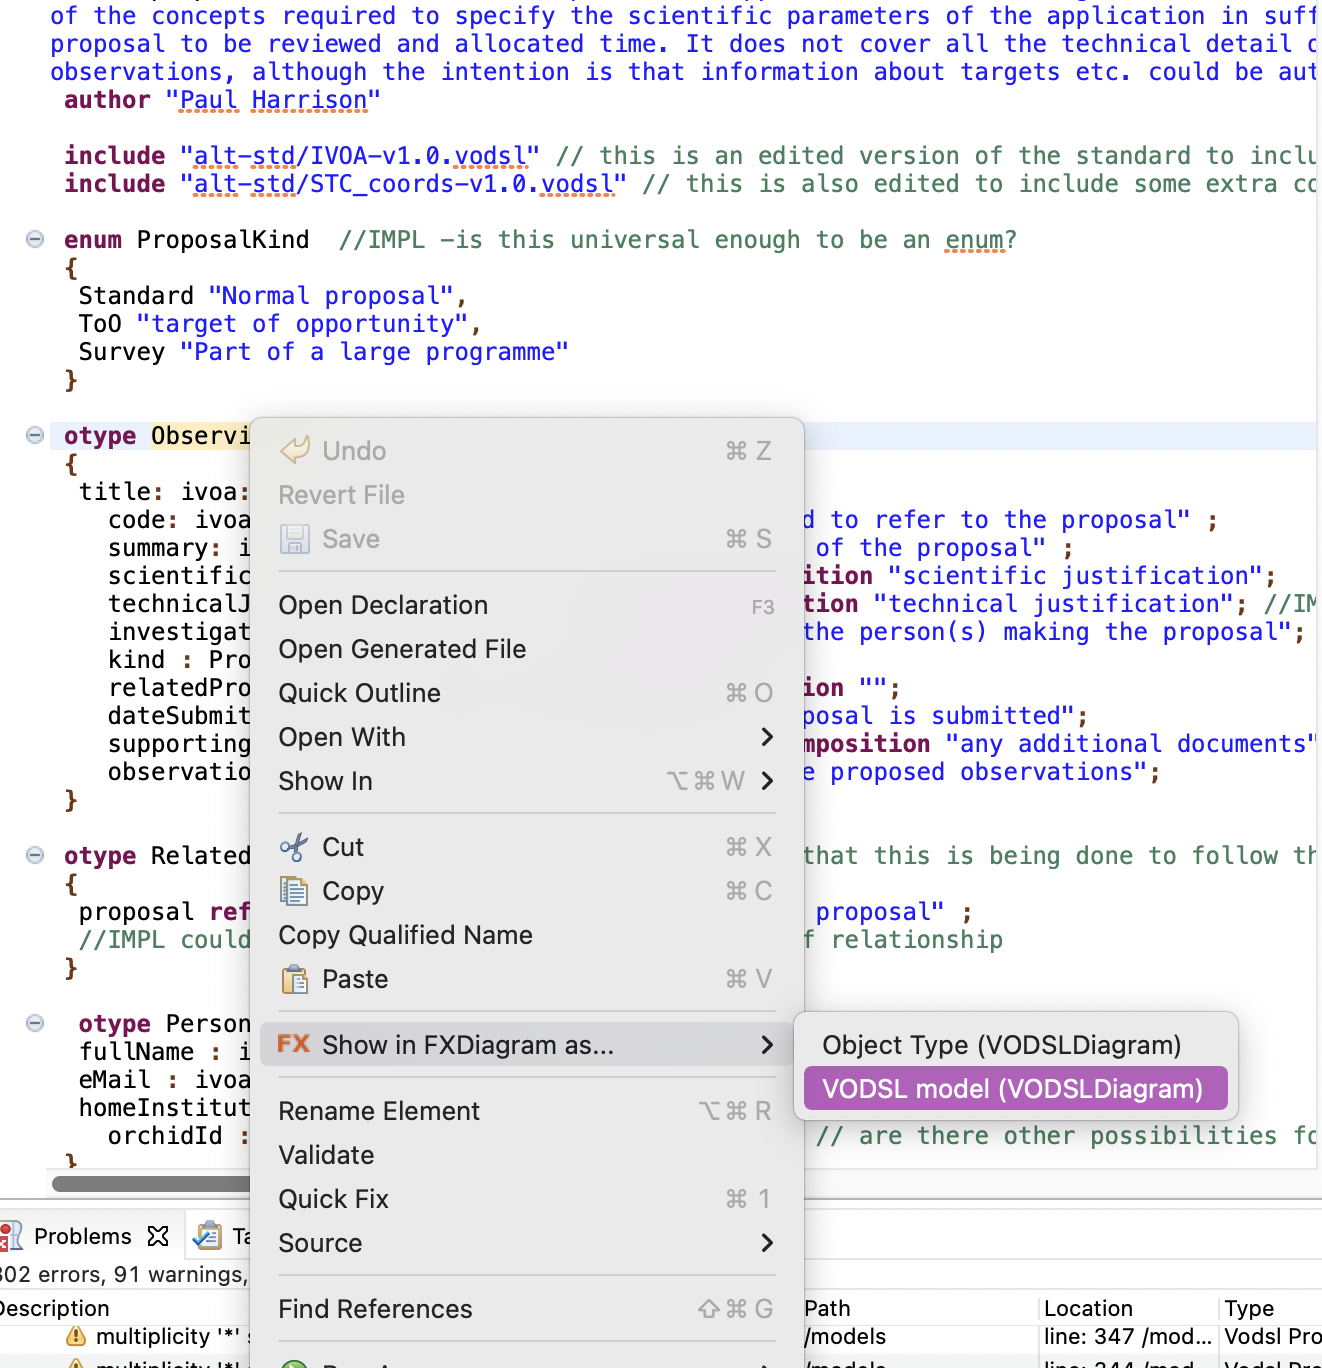
\includegraphics[width=0.5\textwidth]{launchfxdiagram.png}
 
The graphical representation of the model is basically read-only in that it is not possible to edit model features in the graphical window. 
However, as well as visualisation,
it can usefully be used for navigation around the model.


Navigation in the view is possibly a little un-intuitive - on a Mac the following gestures work
\begin{itemize}
\item Panning is done with a two finger drag on trackpad.
\item Zooming is done with a two finger pinch gesture.
\item A menu consisting of a ring of icons can be invoked with a two finger tap - the menu as a range of functions including changing the zoom and saving the diagram.
\item Double-clicking on a model item in the view will select that item in the textual view, 
and conversely, right-clicking in the textual view and chosing "Show in FXDiagram" again will select the item in the graphical view.
\end{itemize}



\subsubsection{Installing the Eclipse plugin}
It is generally recommeded to install the plugin in its own instance of Eclipse (due to some dependencies that are difficult to find)
 rather than using the usual eclipse plugin installation mechanisms in a pre-existing eclipse instance. This can be achieved thus;
 
\begin{enumerate}
  \item ensure that you have a Java 11 or later installed on your machine as well as \href{https://graphviz.org}{graphviz}
\item download the eclipse installer \url{https://www.eclipse.org/downloads/}
\item Run the eclipse installer and select "advanced mode" from the menu at top right.
\item use the green arrow at the top right to add a new user product with the following 
\url{https://raw.githubusercontent.com/pahjbo/vodsl/master/VODSLEditor.setup}
\item select the "VODSL" user product and just click next through the dialogs until you have a running editor.
\item create a new "general" project and then create a file with extension `.vodsl` - eclipse will prompt whether to convert the project to "XText" - say yes.
  
\end{enumerate} 


\subsection{Standalone Compiler}
It is possible to use the parser machinery in a stand-alone fashion (i.e.\ without 
having to use eclipse to edit the vodsl) by using a jar that an be found by followin this link
to \href{https://search.maven.org/search?q=g:%22org.javastro.vodsl%22%20AND%20a:%22vodslparser%22}{maven central}.


Use the following command to run the parser
\begin{lstlisting}[language=bash]
   $ java -jar vodslparser-0.4.5-standalone.jar model.vodsl
\end{lstlisting}

which will produce a file `model.vo-dml.xml` of the equivalent VO-DML.

The capability of converting VODSL to VO-DML on the commandline is also included within the \href{https://github.com/ivoa/vo-dml/tree/master/tools}{VO-DML gradle plugin}.

\appendix
\section{Changes from Previous Versions}

No previous versions yet.  
% these would be subsections "Changes from v. WD-..."
% Use itemize environments.
\section{Full example of VO-DSL}

The following is the full model from which the sections above took snippets.
\begin{lstlisting}[language=vodsl]
/*
 *  created on 25 Feb 2022 
 */
 
 model example (0.1) "description here" 
   author "Paul Harrison"
   author "An Other"
   
   include "IVOA-v1.0.vodsl"
   
package p "top level package" {
	package n "nested package" {
     primitive angle "another primitive"     
	}
}
   
enum options "an enum" {
	val1 "first option",
	val2 "second option"
}   

dtype aQuant -> ivoa:Quantity "an angle quantity" {
			value : p.n.angle  "angle";
}

abstract otype base {
		    q : ivoa:Quantity "a quantity";   
}

abstract otype ad1 -> base "an abstract subtype "{	
}

otype o1 {
	     /* the following attribute is a 'natural key' for the otype */
	       name : ivoa:string iskey "the identifier";
			   bv : ivoa:anyURI  "Description";
		    /* note use of ^ to be able to 
		            re-use reserved word.*/	
		    ^author: ivoa:string "author"; 
}

dtype myQuant -> ivoa:RealQuantity "a flagged quantity" {
			flag : ivoa:boolean "the flag" ;
}

/* it should be noted in this example that
 * @* and @+ are not "recommended" for attributes - it 
   might be better to use composition of otypes - but this is 
   not always the case */
otype multiplicities "the @ sign introduces a multiplicity"
{
	m1 : ivoa:integer @? "0 or 1";
	m2 : ivoa:integer @* "0 or many";
	m3 : ivoa:integer @+ "1 or many";
	m4 : ivoa:integer @[2] "twice (as an array?)";
}

 /*  this referred to otype is not affected by the lifecycle
   of other instances in the model */
 otype ReferedTo { 
 	test1: ivoa:integer "";
 }

/* instances of this contained class will only live
   as long as the containing instance.  */
otype Contained  {
 	test2: ivoa:string "";
 }
 
/* this example references and contains the above types */
otype RCTest { 
	ref references ReferedTo "";
	contained : Contained @+ as composition "";
}

/* an example of subsetting */
otype subs -> base {
	/* note that the requirement to refer to the q attribute of base */
   subset base.q as myQuant; //the type of base.q is a supertype of myQuant
}

/* an example of the syntax for a constraint */
otype constrained {
			val : ivoa:integer "just using a natural language constraint" 
			  < "greater than 5" as Natural> ;
		}


\end{lstlisting}


\section{The VODSL grammar}
\label{sec:grammar}
The XText grammar for the VODSL language is presented below. This is done without any explanation, but people who are familiar with language grammars should
be able to learn information about the VODSL syntax and see the equivalences to the VO-DML meta-model.

\lstinputlisting[language=xtext]{../net.ivoa.vodsl/src/net/ivoa/vodsl/Vodsl.xtext}

% NOTE: IVOA recommendations must be cited from docrepo rather than ivoabib
% (REC entries there are for legacy documents only)

\bibliography{ivoatex/ivoabib,ivoatex/docrepo}


\end{document}
